\chapter{基于加权核判别分析的半监督序回归算法}
\label{chap:wkfdor}

\autoref{chap:introduction}和\autoref{chap:review}中,我们分析了研究半监督序回归问题的重要性以及总结了当前对于半监督序回归问题的研究现状。本章我们将提出一种半监督序回归算法——基于加权核判别分析的半监督序回归算法(Weighted Kernel Fisher Discriminant Analysis for Ordinal Regression, WKFDOR)。首先,我们将给出半监督序回归问题的形式化定义。其次,我们将简单介绍半监督学习。WKFDOR算法是基于KDLOR算法\citep{sun2010kernel}做的半监督扩展,因此我们将介绍KDLOR的算法思想及模型。接着,我们将提出WKFDOR算法。最后,我们将通过实验验证提出的WKFDOR算法的有效性。
%谈一下半监督序回归的motivation

\section{半监督序回归问题定义}
%和有监督序回归问题的定义类似
考虑一个有\(K\)个有序类别的半监督序回归问题,用一个连续的整数集合 \(Z=\{1,2,\dots,K\}\)来表示,整数的值表示相应类别在整个标签集合中的序。在半监督序回归问题中,给定一个包含\(L\)个有标签样例\((X^{l},Y^{l})=\{(x_{1:L},y_{1:L})\}\)和\(N-L\)个无标签样例\(X^{u} = {x_{L+1:N}}\)的训练集,其中\(x_{i} \in \chi \subseteq R^{d}\),\(y_{i} \in Z\)。我们的目标是构造一个半监督序回归模型,通过用训练集来学习,使得该模型可以对测试样例给出一个预测的标签。

\section{半监督学习}
在机器学习中,半监督学习通过在训练的过程中不仅使用有标签数据,同时还使用无标签数据,从而获得比只使用有标签数据训练更好的性能。为了使用无标签数据,需要对数据的分布做一个假设,称为平滑假设(Smoothness Assumption)\citep{chapelle2006semi}。
%[O.Chapelle,B.Scho ̈lkopf,andA.Zien,Semi-SupervisedLearn-ing. MIT Press Cambridge, 2006.]。
基于这个假设,出现了多种半监督学习方法,例如基于图的方法(Graph-based Methods)、低密度分离方法(Low-density Separation Methods)、生成模型(Generative Models)等\citep{zhu2005semi}。
%[X. Zhu, “Semi-supervised learning literature survey,” Technical Report 1530, Department of Computer Sciences, University of Wisconsin, Madison, Tech. Rep., 2006.]。

这里需要指出的是,半监督学习的目标是用训练集训练模型,在应用时预测训练时未出现的新样例的标签。和半监督学习十分类似的一种学习方式称作直推式学习(Transductive Learning,TL),不同的是直推式学习是直接去预测训练集中无标签数据的标签。这里,我们只考虑半监督序回归问题。

\section{KDLOR算法回顾}
基于核判别分析的序回归算法KDLOR\citep{sun2010kernel}是一种高效的有监督序回归技术。KDLOR通过一个序约束来使用序信息,将传统的核判别分析(Kernel Fisher Discriminant Analysis,KFD)方法拓展到序回归问题上。KFD的算法思想和FDA相同,它通过核技巧将FDA扩展到更一般的非线性情况。下面简单介绍FDA算法。

FDA的目标是找到一个投影向量\(w\),使得原始数据通过投影之后可以轻松地被分类。为方便讨论,\autoref{fda_mk}和\autoref{fda_m}、\autoref{fda_Sb}、\autoref{fda_Sw}分别定义类中心、类间协方差矩阵(Between-Class Covariance Matrix)和类内协方差矩阵(Within-Class Covariance Matrix)。 其中,\(m_{k}\)是第 \(k\)个类别样例的均值,\(L_{k}\) 是第\(k\)个类别有标签样例的个数,\(X_{k}\) 是第\(k\)个类别有标签样例的集合。\(m\)是所有类别样例的均值,\(L\) 是有标签样例的个数,\(X\) 所有类别有标签样例的集合。

\begin{equation}
\label{fda_mk}
m_{k}=\frac{1}{L_{k}}\sum_{x\in X_{k}}x
\end{equation}

\begin{equation}
\label{fda_m}
m =\frac{1}{L}\sum_{x \in X} x
\end{equation}

\begin{equation}
\label{fda_Sb}
S_{b} = \frac{1}{L}\sum_{k=1}^{K} L_{k} (m_{k} - m)(m_{k} - m)^{T}
\end{equation}

\begin{equation}
\label{fda_Sw}
S_{w} = \frac{1}{L}\sum_{k=1}^{K}\sum_{x\in X_{k}}(x-m_{k})(x-m_{k})^{T}
\end{equation}

数据在投影后的空间里的分离度可以通过两个指标来定义:投影后的类内协方差,越小越好;投影后的类间协方差,越大越好。要同时满足这两个指标可以通过最小化如下的Rayleigh系数:

\begin{equation}
\label{fda_obj}
J_{w} = \arg \min{\frac{w^{T} S_{w} w}{w^{T} S_{b} w} }
\end{equation}

通过求解\autoref{fda_obj}的优化问题,可以得到最优的投影向量。通过该投影向量,同类数据在投影后的空间里可以分布得很紧凑,同时不同类别的数据在投影后的空间里能够分散开来,从而最小化类别之间的重叠度。核判别分析是一种高效的降维和分类方法,原始数据通过投影之后,可以轻松地被分类(例如通过一个阈值模型)。类中心、类内协方差矩阵、类间协方差矩阵有效地体现了数据的分布特征。

下面我们介绍KDLOR算法的基本思想和模型。KDLOR的基本任务是找到一个可以保存序信息的最佳投影向量。为了保证序的正确性,在映射后的空间,序更高的类的均值要大于序更低的类。此外,为了达到FDA的目标,该投影向量必须保证相邻序的类别之间有大的间隔,同时每个类别内部的数据能够有小的方差。基于这个分析,KDLOR模型在线性情况下的数学形式表示如下:
\begin{equation}
\label{kdlor}
\left\{\begin{array}{rll} \min & J(w,\rho)=w^{T}\cdot S_{w}\cdot w-C\cdot \rho& \\
\\
s.t. & w^{T}\cdot (m_{k+1}-m_{k})\geq\rho,{} \\
     & k = 1,2,\dots,K-1\\
\end{array}
\right.
\end{equation}
其中 \(S_{w} = \frac{1}{L}\sum_{k=1}^{K}\sum_{x\in X_{k}}(x-m_{k})(x-m_{k})^{T}\) 是类间协方差矩阵,\(m_{k}=\frac{1}{L_{k}}\sum_{x\in X_{k}}x\) 是第 \(k\)个类别的样例的均值,\(L\) 是有标签样例的个数,\(X_{k}\) 是第\(k\)个类别的样例集合。该优化问题的目标是找到一个投影向量 \(w\) ,可以满足上文提到的两方面要求。惩罚系数 \(C\)用来平衡目标函数中的两项。如果\(\rho>0\),就可以保证序关系的正确性。非线性情况下模型的形式和上面类似,使用核技巧就可以得到。

由于KDLOR是以核判别分析为基本框架,所以它也可以充分地利用数据分布的信息。而基于支持向量机的序回归算法由于是通过支持向量来决定分类面,所以会忽略数据的全局信息,从而可能导致得到的解不合理\citep{sun2010kernel}。如\autoref{fig_kdlor_fig1}所示,基于最大间隔理论,SVM找到的最优投影向量是\(w\)(相应的分类面垂直于该投影向量)。但是\(w\)忽略了数据的全局分布信息,即没有考虑数据的分布是有一定的规律性。当考虑数据的全局分布信息时,更合理的投影向量应该是\(w^{'}\)。

% \begin{figure*}[!htb]
% %\centering
% {\subfloat[是否考虑类的全局分布情况下的两种投影方向。其中$w$是仅考虑最大间隔的投影,$w^{'}$考虑了类的全局分布。]{\includegraphics[width=3in]{figures/kdlor_fig1}%
% \label{fig_kdlor_fig1}}}
% %\hfil
% %\subfloat[加权策略估计的类中心情况]{\includegraphics[width=3in]{figures/kdlor_fig2}%
% %\label{fig_kdlor_fig2}}}
% \caption{合成数据集的数据分布情况和投影结果。$x^{1d}$ 和 $x^{2d}$ 分别对应样例的两个属性;$p^{l}(x)$是KDLOR算法的投影函数,其中$\alpha_{i}^{l}$是第$i$个有标签样例的系数。}
% \label{fig_kdlor_analysis}
% \end{figure*}

\begin{figure}[htb]
   \centering
   \includegraphics[width=4.5in]{figures/kdlor_fig1}
\caption{是否考虑类的全局分布情况下的两种投影方向\citep{sun2010kernel}。其中$w$是仅考虑最大间隔的投影,$w^{'}$考虑了类的全局分布。}
\label{fig_kdlor_fig1}
\end{figure}

此外,相比较于一些流行的有监督序回归方法,KDLOR不仅可以获得很有竞争力的分类性能同时也有相对最低的计算复杂度\citep{sun2010kernel}。
%Besides, KDLOR has the smallest problem size (i.e., at most L [7]) in comparison to the ap- proaches in [1–5]. 
但是,当有标记数据很少的时候,有监督序回归方法就会受到限制。对于KDLOR来说,这个限制就是类的中心趋势难以准确地估计。

\section{基于加权核判别分析的半监督序回归技术}

根据上一节对KDLOR的介绍和分析,我们考虑将其拓展到半监督形式,从而利用无标签数据来提升性能。值得注意的是,由于序信息的存在,已有的半监督学习模型难以直接应用到序回归问题上。

对于基于FDA的方法,用训练数据估计类中心和协方差矩阵的准确性将对序回归模型的性能产生重要的影响。而当有标签数据很少的时候,仅用有标签数据很难准确地估计类分布。因此,我们考虑利用存在的无标签数据来更准确地估计类分布。本节我们提出了一种半监督核判别分析序回归技术——WKFDOR。具体的说,我们首先估计无标签数据对于每个类别的隶属度(Membership),其次通过一个加权策略来计算整个训练集(包括有标签数据和无标签数据)上的类分布,再将这个加权类分布应用到KDLOR框架下得到最终模型。下面先介绍计算无标签数据隶属度的方法,再介绍我们提出的WKFDOR算法。

\subsection{估计无标签数据对每个类别的隶属度}
这里我们使用一个标签传播(Label Propagation)的方法\citep{zhou2004learning}
%[D. Zhou, O. Bousquet, T. N. Lal, J. Weston, and B. Scho ̈lkopf,“Learning with local and global consistency,” in Advances in Neural Information Processing Systems 16. MIT Press, 2004, pp. 321–328.])
来估计无标签数据对于每个类别的隶属度。\autoref{alg_mem}列出了\textit{mConsistency}算法的主要步骤。

\IncMargin{1em}
\begin{algorithm}
\SetKwData{Left}{left}\SetKwData{This}{this}\SetKwData{Up}{up}
\SetKwFunction{Union}{Union}\SetKwFunction{FindCompress}{FindCompress}
\SetKwInOut{Input}{input}\SetKwInOut{Output}{output}
\Input{有标签数据 $(X^{l},Y^{l})=\{(x_{1:L},y_{1:L})\}$; \\
 无标签数据$X^{u}=\{(x_{L+1:N})\}$}
\Output{隶属度矩阵 $U=(u_{jk})_{N \times K}$}
\BlankLine
\emph{$Y_{N \times K}$ $\leftarrow$ $Y_{jk}=\begin{cases}1,\; y_{j}=k \\0,\; otherwise\end{cases}$}\;
\emph{$W_{N \times N}$ $\leftarrow$ $W_{ij}=\begin{cases}\exp(-\|x_{i}-x_{j}\|^{2}/2\varepsilon^{2}),\; i\neq j \\0,\; otherwise\end{cases}$}\;
\emph{$S=D^{-1/2}WD^{-1/2}$,$D$是一个对角矩阵,$D_{ii}=\sum_{j=1}^{N}W_{ij}$}\;
\emph{$F^{*}=(1-\alpha)(I-\alpha S)^{-1}Y$, $\alpha\in(0,1)$}\;
\emph{$F^{n}_{N \times K}$ $\leftarrow$ $F^{n}_{jk}=F^{*}_{jk}/\sum_{k=1}^{K}F^{*}_{jk}$}\;
\emph{$U$ $\leftarrow$ $u_{jk}=\begin{cases}Y_{jk},\; x_{j}\in X^{l} \\F^{n}_{jk},\; x_{j}\in X^{u}\end{cases}$}\;
\caption{mConsistency}\label{alg_mem}
\end{algorithm}
\DecMargin{1em}

该算法的主要思想是,通过让每一个数据点迭代地传播它的标签信息给邻近点,直到达到一个全局稳定的状态\citep{zhou2004learning}。其形式化表示是\(F(t+1)=\alpha SF(t)+(1-\alpha)Y\),参数\(\alpha\)用来平衡标签信息的扩散(第一项)和原始状态的维持(第二项),\(Y\)是初始标签矩阵,\(S\)是对邻近度矩阵(Affinity Matrix)\(W\)的对称归一化。迭代过程会收敛到\(F^{*}=(1-\alpha)(I-\alpha S)^{-1}Y\)\citep{zhou2004learning},所以标签传播的最终状态可以直接通过\(F^{*}\)来计算。

由于标签信息是通过数据点之间的邻近度矩阵来扩散的,所以该算法可以被看作是一种基于图的半监督学习方法。对每个无标签数据点\(x_{i}\),它最终接收到的标签信息存储在一个行向量\(F^{*}_{i}=[F^{*}_{i1},\dots,F^{*}_{iK}]\)里。根据平滑假设,\(F^{*}_{i}\)可以表示\(x_{i}\)属于每个类别的置信度(Confidence)。因此,我们归一化\(F^{*}\)并把它作为隶属度矩阵,表示为 \(U=(u_{jk})_{N \times K}\)。这里需要指出的是,有标签数据的隶属度直接从给定的标签\(Y^{l}\)得到,具体请参\autoref{alg_mem}中的步骤6。

\textit{mConsistency}算法简单且快速,它的主要计算开销是一个矩阵求逆和一个矩阵乘法操作,时间复杂度是\(O(N^{3})\),其中\(N\)是训练样例的个数。

\subsection{基于加权核判别分析的半监督序回归技术}
为了利用无标签数据来提升对类分布估计的准确性,我们使用一个加权策略来计算类均值和类内协方差矩阵。考虑到实际应用中的数据往往在原始空间是非线性的,所以我们在这里使用了核技巧。具体的做法是:首先通过一个非线性映射函数 \(\phi\),将原始数据映射到一个更高维度的空间 \(\mathcal{F}\),使得数据在该空间是线性可分的;接着类似于线性情况下的做法,在映射后的数据上求得最优的投影向量。

将原始空间映射到 \(\mathcal{F}\)之后,加权类中心(Weighted Class Means)和加权类内协方差矩阵(Weighted Within-Class Covariance Matrix)定义如下:
\begin{gather}
\label{weighted_mean}
m^{\phi}_{k}=\frac{\sum_{j=1}^{N} u_{jk}\phi(x_{j})}{\sum_{j=1}^{N} u_{jk}} \\
\label{weighted_cov}
S^{\phi}_{w}=\frac{1}{u} \sum_{k=1}^{K} \sum_{j=1}^{N} u_{jk}(\phi(x_{j})-m^{\phi}_{k})(\phi(x_{j})-m^{\phi}_{k})^{T}
\end{gather}
其中所有的训练数据(包括有标签和无标签样例)都被用来估计类分布。 \(u=\sum_{k=1}^{K} \sum_{j=1}^{N} u_{jk}\),\(u_{jk}\)是 \(x_{j}\)属于第\(k\)个类别的隶属度。通过\autoref{weighted_mean}和\autoref{weighted_cov}可以看到,那些对某个类别有更高隶属度的数据点将会对该类的类中心和类内协方差矩阵贡献更大。这两个类分布的特征分别反映了类的中心趋势和类的分布形状,无标签数据的贡献有助于更准确地估计它们,从而更好地决策最优的投影向量。假设对所有无标签数据的隶属度的估计都完全正确的话(即当\(x_{j}\)的真实标签是\(k\)时, \(u_{jk}=1\) 而\(u_{jk^{c}}=0,\;k^{c}\neq k\)),通过该加权策略,相当于额外使用了\(N-L\)个有标签数据来计算类分布,这毫无疑问会比仅使用少量的有标签数据更加准确。

%翻译 lie in the span of
下面,我们将详细推导基于加权核判别分析的半监督序回归(WKFDOR)模型的数学形式。根据再生核理论(Reproducing Kernels Theory),任何解 \(w\in \mathcal{F}\)必须要满足如下形式:
%在所有在(\mathcal{F}\)中的训练样例形成的
\begin{equation}
\label{kernel_w}
w=\sum_{i=1}^{N}\alpha_{i}\phi(x_{i}),\quad \alpha_{i} \in R
\end{equation}
其中 \(\alpha_{i}\) 是第\(i\)个样例的系数。通过投影向量\(w\),在映射后的空间里,加权类中心和加权类内协方差矩阵由下面公式计算:
\begin{gather}
\label{project_mean}
w^{T} \cdot m^{\phi}_{k}=\alpha^{T} \cdot \mathcal{M}_{k} \\
\label{project_cov}
w^{T} \cdot S^{\phi}_{w} \cdot w=\alpha^{T} \cdot \mathcal{N} \cdot \alpha
\end{gather}
其中\(\alpha=[\alpha_{1},\alpha_{2},\dots,\alpha_{N}]^{T}\)。\(\mathcal{M}_{k}\)是一个\(N \times 1\)的列向量,其中
\begin{equation}
\label{M}
(\mathcal{M}_{k})_{i}=\frac{1}{u_{k}}\sum_{j=1}^{N}u_{jk}  k(x_{i},x_{j})
\end{equation}
\(\mathcal{N}\) 是一个\(N\times N\) 的矩阵,如下计算:
\begin{equation}
\label{N}
\mathcal{N}=\frac{1}{u}\mathcal{K}\cdot[\sum_{k=1}^{K}(D_{k}-D_{k} \cdot \mathbf{1}_{u_{k}} \cdot D_{k})]\cdot \mathcal{K}
\end{equation}
\(\mathcal{K}=(k(x_{i},x_{j}))_{N \times N}\)表示核矩阵(Kernel Matrix),其中\(k(\cdot,\cdot)\)是核函数(Kernel Function)。\(D_{k}\)是一个对角矩阵,对角线元素 \((D_{k})_{ii}=u_{ik}\)。\(\mathbf{1}_{u_{k}}\) 是一个所有项都等于\(1/u_k\)的矩阵,其中\(u_{k}=\sum_{j=1}^{N}u_{jk}\)。

WKFDOR算法的目标是找到一个最优的投影向量,使得在映射后的空间里,同类数据点能够相聚紧凑,并且相邻类别的数据点可以分隔开,同时能够保证序的正确性。通过上面的推导和分析,WKFDOR算法的数学形式描述如下:
\begin{equation}
\label{wkfdor}
\left\{\begin{array}{rll} \min & J(\alpha,\rho)=\alpha^{T}\cdot \mathcal{N}_{\mu} \cdot \alpha-C\cdot \rho& \\
\\
s.t. & \alpha^{T}\cdot (\mathcal{M}_{k+1}-\mathcal{M}_{k})\geq\rho,{} \\
     & k = 1,2,\dots,K-1\\

\end{array}
\right.
\end{equation}
为了保证矩阵\(\mathcal{N}\)是正定的( Positive Definite), 令\(\mathcal{N}_{\mu}=\mathcal{N}+\mu I\),其中
\(I\)是单位矩阵。

通过拉格朗日乘数法(Lagrange Multipliers),可以将WKFDOR模型转化成一个有线性约束的二次规划问题(Quadratic Programming,QP),而该问题能够很容易得到求解。需要指出的是,通过投影向量映射后的空间是一个一维空间。求解出\(\alpha\)之后(相当于得到最优投影向量\(w\),由于在核函数的作用下,我们无需显式地计算出\(w\)),相邻类别之间的阈值根据下式计算:
\begin{equation}
\label{threshold_wkfdor}
b_{k}=\begin{cases}
\frac{\alpha^{T} \cdot (u_{k+1} \mathcal{M}_{k+1} + u_{k} \mathcal{M}_{k})}{u_{k+1}+u_{k}},\quad &k \in \{1,2,\dots,K-1\} \\
+\,\infty,\quad &k=K
\end{cases}
\end{equation}
注意,\autoref{threshold_wkfdor}定义的阈值是在映射后的空间里。可以看出,这些阈值是由有标签数据和无标签数据共同决定的。对于测试样例\(x\),其投影结果是:
\begin{equation}
\label{projResult_wkfdor}
p(x)=w^{T} \cdot \phi(x)=\sum_{i=1}^{N} \alpha_{i} k(x_{i},x)
\end{equation}
最后,我们可以根据下面的规则预测 \(x\) 的序:
\begin{equation}
\label{rank_rule_wkfdor}
r(x)=\min \limits_{k \in \{1,2,\dots,K\}} \{k\mid p(x)-b_{k}<0\}
\end{equation}

不同于KDLOR算法,WKFDOR算法不仅使用了有标签数据,同时还利用了无标签数据来估计类均值和类内协方差矩阵。我们通过计算隶属度(\autoref{alg_mem})和加权策略来使用这些无标签数据。由于在实际应用中通常存在大量的无标签数据,所以合理利用它们能够更加准确地估计潜在的数据分布。因此,我们提出的WKFDOR算法能够在KDLOR的基础上获得一个更好的性能。下一节中,我们将会通过实验来验证算法的有效性。

\section{实验验证}
为了验证我们提出的WKFDOR算法能够通过加权策略有效地使用无标签数据,我们设计了两组实验。首先,我们在人工合成的数据集上比较WKFDOR算法和KDLOR算法,并对结果可视化。其次,我们在10组真实的有序数据集上评估WKFDOR算法和KDLOR算法的性能。

\subsection{实验设置}
\label{wkfdor_expSet}
本实验采用下面的高斯核函数来做非线性映射:
\begin{equation}
\label{Gaussian_kernel}
k(x,y)=\exp(-\frac{\parallel x-y \parallel^{2}}{2\sigma^{2}})
\end{equation}
KDLOR算法的超参数\(\mu\)、\(C\)、 \(\sigma\),以及\textit{mConsistency}算法的超参数\(\alpha\)、\(\varepsilon\) 通过五折交叉验证(5-Fold Cross Validation)来确定。在这里,WKFDOR算法的\(\mu\)、\(C\)、 \(\sigma\)采用和KDLOR算法相同的值。使用相同的超参值来比较这两个算法看上去是公平的,但实际上WKFDOR算法可能存在更优的参数设置。

对于所有的数据集,我们采用统一的数据预处理方法。我们采用0-1编码来处理数据集中的离散属性,并使用z-score方式来做归一化(即将数据归一化成\((0,1)\)高斯分布)。
% 数据预处理:对于离散属性(categorical)通过0-1编码来处理,使用z-score归一化数据(归一化成(0,1)高斯分布)

\subsection{合成数据集}
为了可视化和便于理解算法的学习效果,我们在这一小节中生成了一个二维数据集。该数据集共有4个类别,每个类别从一个二元高斯分布中生成50个样例。按照序从小到大,将这4个高斯分布的中心依次设置为(10,10)、(30,20)、 (20,10) 和(40,20),并将它们的标准差都设置为(2,2)。对每一个类别,随机抽取25个样例作为测试数据,剩下的25个样例作为训练数据。再从训练数据中随机抽取5个作为有标签数据,剩下的20个作为无标签数据。数据的分布情况见\autoref{syn_labeled},可以看出这是一个非线性的序回归问题。

在该实验中,我们在合成数据集上比较WKFDOR算法和KDLOR算法,其中无标签数据对于每个类别的权重通过\textit{mConsistency}算法计算得到。\autoref{syn_data}展示了训练数据的分布情况和算法的投影结果。\autoref{syn_labeled}画出了只用有标签数据估计的类中心,可以看出它们和用整个数据集计算得到的类中心相距甚远,这是因为有标签数据量很少,难以准确估计。而\autoref{syn_weightedMeans}画出的加权类中心更加靠近于用整个数据集估计的类中心,这说明了我们提出的加权策略以及 \textit{mConsistency}算法是行之有效的。\autoref{kdlor_proj}和\autoref{wkfdor_proj}分别展示了KDLOR算法和WKFDOR算法得到的投影结果,其中五角星表示类别之间的阈值。对于KDLOR算法,有标签数据的投影可以按照序很好地分开,而测试数据在投影后的空间里相邻类别之间有严重的重叠,即对测试数据的序预测不准确。相反,对于WKFDOR算法,有标签数据和测试数据的投影都能够按照序很好地分开,尤其对测试数据的预测结果有显著的提升。合成数据集的实验结果说明,我们提出的WKFDOR算法能够有效地利用无标签数据从而提升处理序回归问题的性能。

\begin{figure*}[!htb]
%\centering
{\subfloat[有标签数据在原始空间的分布情况]{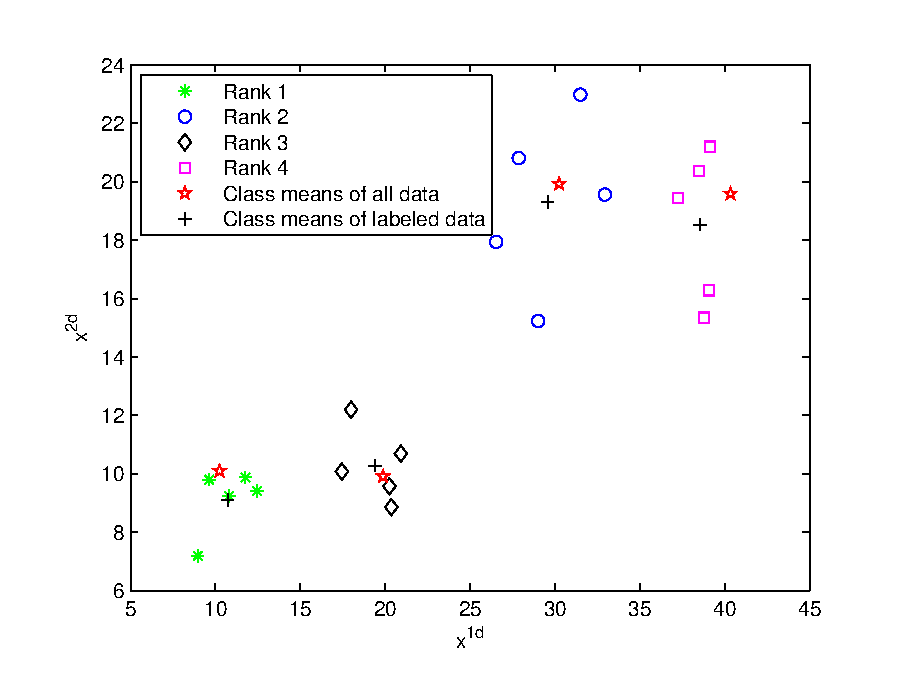
\includegraphics[width=3in]{figures/syn_labeled3}%
\label{syn_labeled}}
\hfil
\subfloat[加权策略估计的类中心情况]{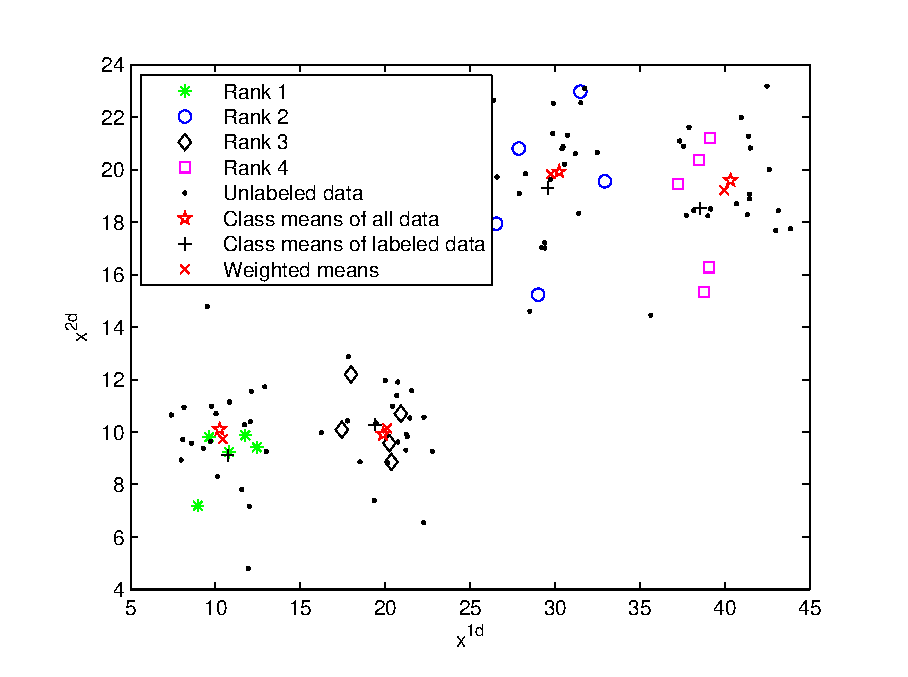
\includegraphics[width=3in]{figures/syn_weightedMeans3}%
\label{syn_weightedMeans}}
\hfil
\subfloat[KDLOR算法的投影结果]{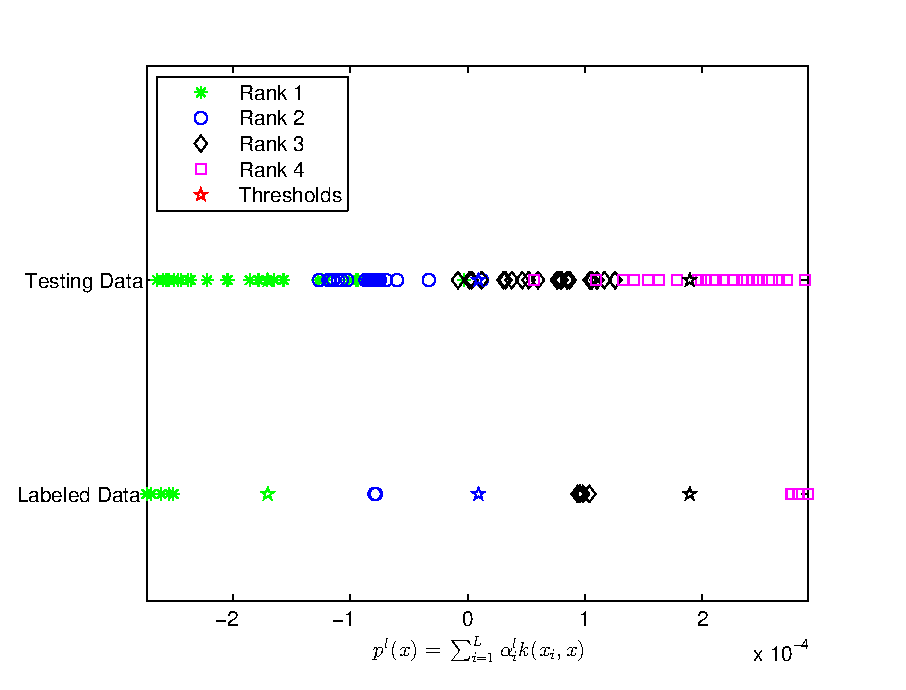
\includegraphics[width=3in]{figures/kdlor_proj3}%
\label{kdlor_proj}}
\hfil
\subfloat[WKFDOR算法的投影结果]{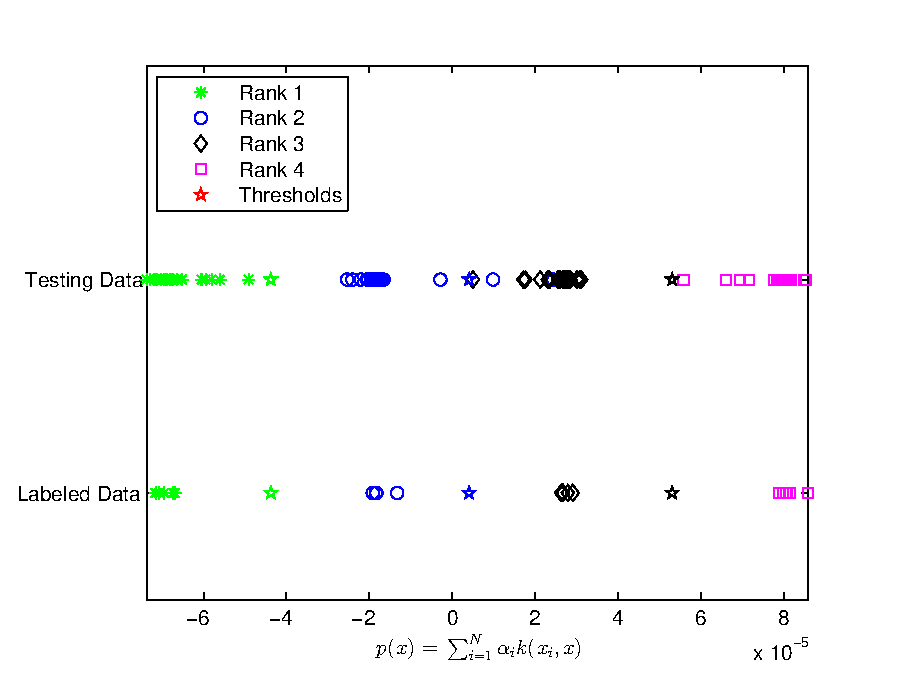
\includegraphics[width=3in]{figures/wkfdor_proj3}%
\label{wkfdor_proj}}}
\caption{合成数据集的数据分布情况和投影结果。$x^{1d}$ 和 $x^{2d}$ 分别对应样例的两个属性;$p^{l}(x)$是KDLOR算法的投影函数,其中$\alpha_{i}^{l}$是第$i$个有标签样例的系数。}
\label{syn_data}
\end{figure*}

\subsection{真实数据集}
\label{wkfdor_realData}

\begin{table}[!htbp]
\caption{真实数据集}
\label{table_realSets}
\centering
\begin{tabular}{l|cccc}
\toprule
Datasets & \# Attributes & \# Ranks & \# Training & \# Testing\\
\midrule
TAE & 5 & 3 & 100 & 51\\
Thyroid-new & 5 & 3 & 130 & 85\\
Balance & 4 & 3 & 400 & 225\\
Car & 6 & 4 & 160 & 100\\
SWD & 10 & 4 & 600 & 400\\
LEV & 4 & 5 & 600 & 400\\
ESL & 4 & 9 & 300 & 188\\
ERA & 4 & 9 & 600 & 400\\
Sushi & 17 & 5 & 7000 & 3000 \\
Connect-4 & 42 & 3 & 7000 & 3000\\
\bottomrule
\end{tabular}
\end{table}

% 可以详细描述一下数据集
在这一小节中,我们使用10个真实的有序数据集(见\autoref{table_realSets})来比较WKFDOR算法和KDLOR算法。TAE、Thyroid-new、Balance、Car、Connect-4取自UCI机器学习库(UCI Machine Learning Repository)\footnote{Car和Connect-4分别从原始数据集随机抽取一部分样例用于本实验。}\citep{Bache+Lichman:2013}。
%[M. Lichman, “UCI machine learning repository,” 2013. [Online]. Available: http://archive.ics.uci.edu/ml]。
SWD、LEV、ESL、ERA是真实的人类决策数据集,其中属性和标签都是有序值\citep{ben2006generating}。
%[A. Ben-David and L. Sterling, “Generating rules from examples of human multiattribute decision making should be simple,” Expert Systems with Applications, vol. 31, no. 2, pp. 390–396, 2006.]。
Sushi数据集\citep{kamishima2009efficient}是通过问卷调查获取的用户对各种寿司的偏好程度数据。其中我们综合了用户属性数据和寿司属性数据,并剔除了不完整的样例(比如用户A对寿司B没有填写偏好程度,则删除该行数据),再从中随机抽取10000个作为我们的实验数据。

对于每个数据集,取一半的训练数据作为有标签数据,剩下的一半作为无标签数据。分别将WKFDOR算法和KDLOR算法在每个数据集上跑20遍,统计MAE和MZE的平均值和标准差。具体结果见\autoref{table_realResults20m}。

MAE指标中,WKFDOR算法在6个数据集上结果的均值要优于KDLOR算法,其中在2个数据集上(Balance、Connect-4)显著优于KDLOR算法。MZE指标中,WKFDOR算法在9个数据集上结果的均值优于KDLOR算法,并在3个数据集上(Balance、Sushi、Connect-4)显著优于KDLOR算法。整体来看,WKFDOR算法在处理序回归问题时具有更优的性能,尤其是MZE指标。

在真实的序回归问题中,有标签数据缺乏往往导致学习器训练不够,从而在遇到新的测试数据时不能正确地进行预测。WKFDOR算法通过加权策略利用无标签数据来更准确地估计类分布,从而获得更优的泛化性能。该实验中,WKFDOR算法得到的MZE结果几乎都优于KDLOR算法,而在一些数据集上的MAE结果没有体现出优越性,原因可能是\textit{mConsistency}算法对这些数据集中无标签数据属于每个类别的权重估计得不够准确。\textit{mConsistency}算法没有考虑数据的序关系,更偏向于以准确率为目标进行信息传播。例如,有一个真实序为3的点,它到序为1和4的类的距离相同,算法可能会得到该点以相同的置信度属于类别1和4。而在序回归问题中,如果预测该点属于类别4的置信度大于属于类别1的置信度将更有建设性,因为将其预测为4的代价通常会小于预测为1的代价(即MAE所追求的差值最小)。因此,我们将在后面的章节中提出改进的算法,使其在计算权重时考虑序信息并且估计得更加准确,从而提升性能。

%记得加上统计测试的结果*
\begin{table*}[!h]
\caption{KDLOR和WKFDOR在真实数据集上的测试结果。该结果是由运行20次的均值和方差组成,包括MAE和MZE两个指标。每组数据集的最优均值用粗体来表示。用秩和检验(Wilcoxon Rank-Sum Test)做统计测试,其中显著性水平设为0.05,表中显著优于KDLOR的结果用$*$号来标记。}
\label{table_realResults20m}
\centering
\begin{tabular}{l|cc|cc}
\toprule
 & \multicolumn {2}{c|}{MAE} & \multicolumn {2}{c}{MZE} \\
 \cmidrule {2-5}
Datasets & KDLOR & WKFDOR & KDLOR & WKFDOR\\
\midrule
TAE &  {\bf 0.5402$\pm$0.0746} &  0.5471$\pm$0.0648 & 0.5392$\pm$0.0743 & {\bf 0.5353$\pm$0.0630} \\
Thyroid-new & 0.2788$\pm$0.0717 &  {\bf 0.2182$\pm$0.0576} & 0.2741$\pm$0.0736 & {\bf 0.2100$\pm$0.0619} \\
Balance & 0.4829$\pm$0.0427 &  {\bf 0.3109$\pm$0.0244}$^{*}$ & 0.4829$\pm$0.0427 & {\bf 0.3107$\pm$0.0244}$^{*}$ \\
Car & 0.3170$\pm$0.0546 &  {\bf 0.2760$\pm$0.0672} & 0.3070$\pm$0.0517 & {\bf 0.2740$\pm$0.0657} \\
SWD & {\bf 0.5740$\pm$0.0403} &  0.5833$\pm$0.0155 & 0.5097$\pm$0.0341 & {\bf 0.5060$\pm$0.0099} \\
LEV & {\bf 0.6447$\pm$0.0311} &  0.6570$\pm$0.0454 & 0.5307$\pm$0.0235 & {\bf 0.5142$\pm$0.0300} \\
ESL & {\bf 0.4415$\pm$0.0428} &  0.4660$\pm$0.0501 & {\bf 0.4436$\pm$0.0370} & 0.4553$\pm$0.0459 \\
ERA & 1.7706$\pm$0.1889 &  {\bf 1.7005$\pm$0.1524} & 0.8015$\pm$0.0256 & {\bf 0.7891$\pm$0.0238} \\
Sushi & 1.0210$\pm$0.0149 & {\bf 1.0132$\pm$0.0140} & 0.7254$\pm$0.0252 & {\bf 0.7002$\pm$0.0216}$^{*}$ \\
Connect-4 & 0.4982$\pm$0.0087 & {\bf 0.4828$\pm$0.0112}$^{*}$ & 0.4505$\pm$0.0094 & {\bf 0.3752$\pm$0.0097}$^{*}$ \\
%Connect-4 & 0.498183$\pm$0.008699 & 0.482817$\pm$0.011204 & 0.450467$\pm$0.009402 & 0.375200$\pm$0.009743 \\
\bottomrule
\end{tabular}
\end{table*}

\section{小结}
本章我们首先介绍了半监督序回归问题的形式化定义,和有监督序回归问题类似,半监督序回归问题的不同之处在于考虑同时使用有标签数据和无标签数据来训练模型。根据对半监督序回归问题和已有主流有监督序回归技术的分析,我们提出了一种半监督序回归技术——WKFDOR算法。该算法的主要思想是利用无标签数据来更准确地估计类的分布信息,从而获得更优的性能。通过在合成数据集和真实序回归数据集上的实验,我们验证了WKFDOR算法的有效性。








